\chapter{Webové rozhraní} \label{chap:web_page}

Hlavním výstupem této práce je grafická vizualizace pro přehledné zobrazení veškerých dat a komunikaci s uživatelem. Za účelem této prezentace naměřených dat a modelů byla zvolena vizualizace ve formě webové stránky. Webová stránka je dostupná na veřejné IP adrese 147.228.124.68:8881 a její struktura je rozdělena do tří hlavních podstránek. Základem webu je horní horizontální menu, které se skládá z těchto tří tlačítek a uživateli umožňuje proklikávání mezi jednotlivými stránkami.

\begin{table}[h!]
\centering
\begin{tabular}{|P{2.5cm}|P{2.5cm}|P{2.5cm}|} 
 \hline
 Overview & Analytics & About \\
 \hline
\end{tabular}
\end{table}

Z hlediska webového designu mají tlačítka v horizontálním menu úmyslně šedý odstín barvy písma (oproti bílému fontu ve zbytku stránky). Odlišují se tím tlačítka a text, na který není možné klikat. Jednotlivá tlačítka se po přejetí kurzorem mírně zvětší a nabádají uživatele ke kliknutí. \textit{Overview} je stránka, která uživateli poskytuje kompletní a stručný přehled o veškerém dění v chytré domácnosti. Stránka \textit{Analytics} umožňuje interakci s uživatelem, nabízí detailní informace o stavech jednotlivých senzorů a zobrazuje grafy ilustrující očekávané hodnoty v průběhu dne na základě klasifikace pomocí natrénovaného modelu. \textit{About} je doplňující stránka, která velmi stručně popisuje tento projekt a dodává vysvětlivky k ikonám na webu. \par
První akce, kterou webová stránka po zobrazení v internetovém prohlížeči vykoná, je načtení dat ze souboru \textit{webpage\_data.json}. V tomto souboru jsou uloženy poslední hodnoty měřených veličin. Význam tohoto datového souboru je v okamžitém zobrazení posledních hodnot po načtení stránky bez nutnosti čekání, než senzory odešlou data. Hlavní význam to má u senzorů, které odesílají data na základě události (více v \cref{subsec:event_based_msg}) - například změna stavu okna (otevřené nebo zavřené) se děje jen několikrát denně a kdyby webová stránka neměla k dispozici soubor \textit{webpage\_data.json}, pro zobrazení stavu okna by uživatel musel počkat, než se tento stav změní a je odeslán přes broker a engine na webovou stránku. Po obnovení webové stránky by se poslední hodnota opět ztratila. Soubor \textit{webpage\_data.json} je používán pouze při prvotním načtením webu, od této chvíle už webový klient přijímá aktuální hodnoty přes Websocket.  

\section{Programování frontendu} \label{sec:frontend}
Webová stránka byla naprogramována v \textit{HTML} s využitím \textit{JavaScriptu} a kaskádových stylů \textit{CSS}. Struktura kódu je rozdělena podle tří hlavních stránek. Každá stránka má svůj soubor s JavaScriptovým kódem a CSS souborem se styly. JavaScript je zde využitý pro zajištěný potřebných funkcionalit webu - například nově příchozí zpráva se automaticky propíše do požadovaného místa, při uživatelské volbě parametrů pro načtení natrénovaných modelů JavaScript zobrazuje data v požadovaném místě nebo JavaScript mění ikony statusu senzorů podle změn těchto statusů. V CSS souborech je nadefinován design webu. Jsou zde uloženy parametry pro vykreslení dlaždic - barvy, fonty, rozměry a rozmístění na stránce. Kombinací těchto tří nástrojů bylo dosaženo interaktivní webové vizualizace pro prezentaci naměřených dat v projektu chytré domácnosti.

\section{Overview} \label{sec:overview}

Overview je podstránka, která se načte jako výchozí při návštěvě webu. V záhlaví stránky se zobrazuje aktuální čas a datum a pod pruhem s těmito informace se nacházejí dlaždice obsahující informace o naměřených hodnotách. Na \cref{fig:web_overview} je zobrazen náhled stránky Overview. 

\begin{figure}[H]
  \centering
  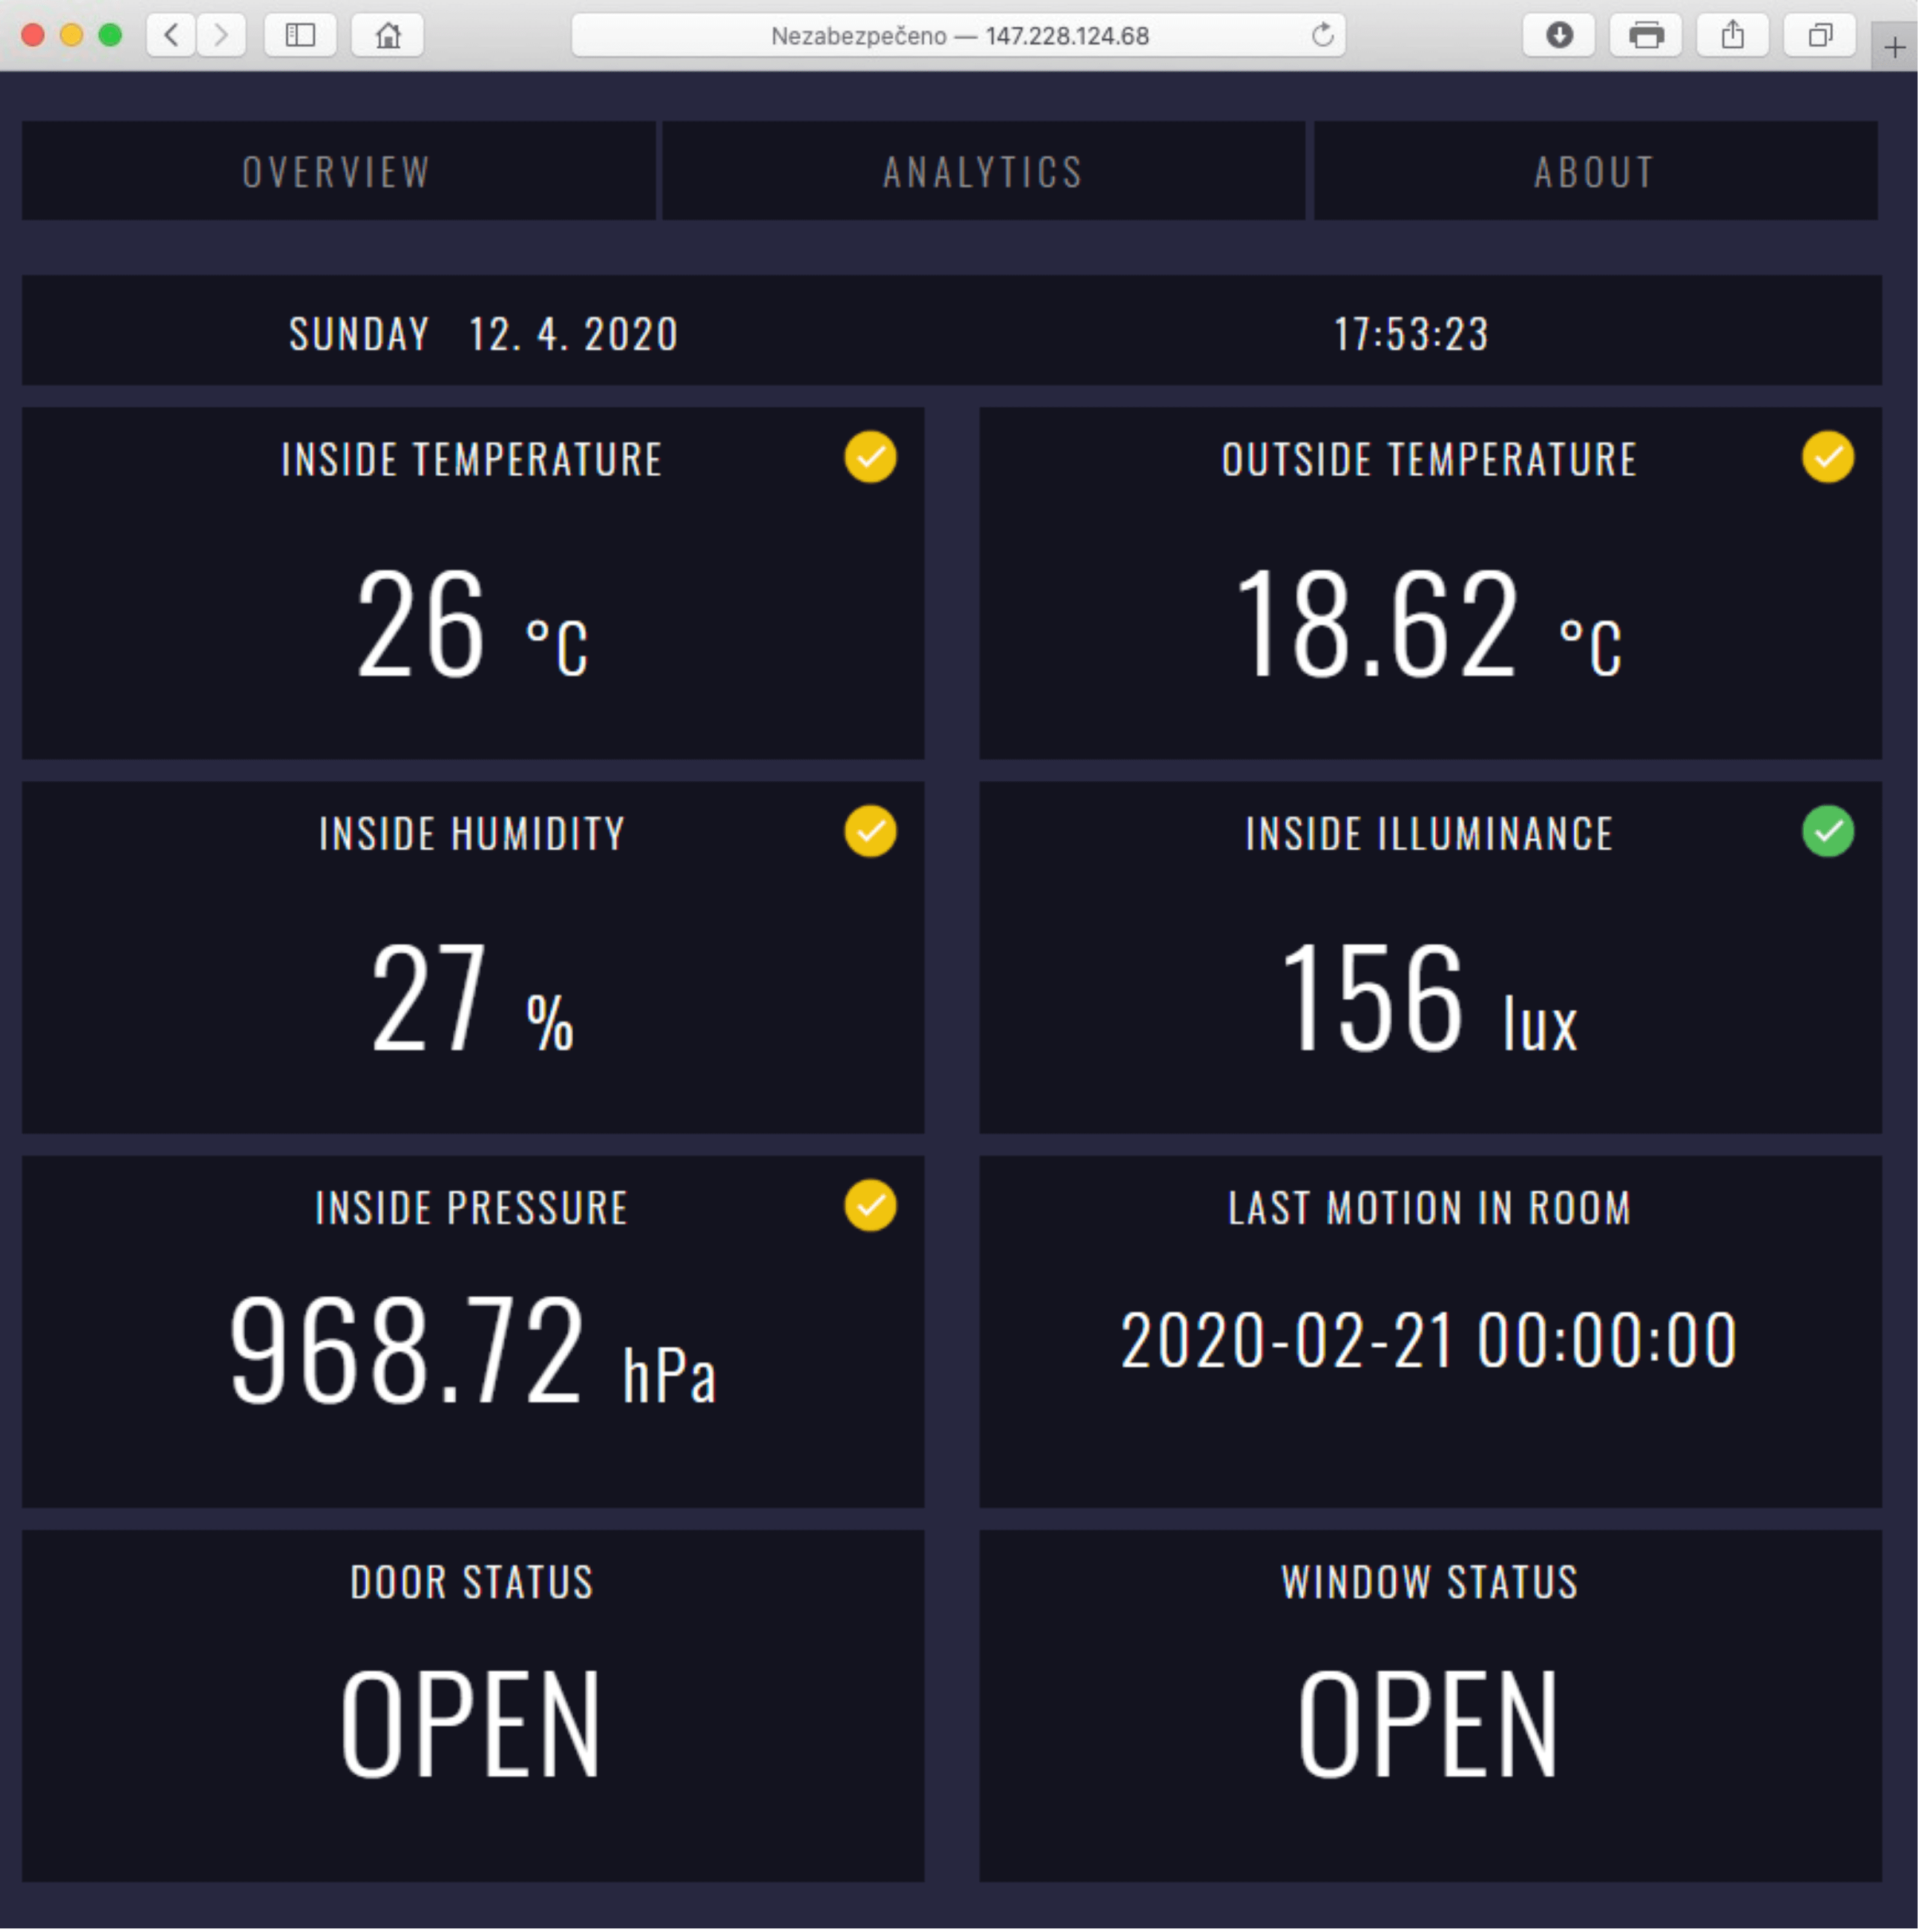
\includegraphics[width=0.8 \textwidth]{web_overview.png}
  \caption{Stránka Overview ve webovém rozhraní}
  \label{fig:web_overview}
\end{figure}  

Šablona dlaždice (\cref{fig:web_overview_tile}) je pro každou veličinu stejná - skládá se z názvu měřené veličiny, ikony zobrazující stav senzoru (více v \cref{subsec:diagnostics_output}) a číselné hodnoty s fyzikální jednotkou.

\begin{figure}[H]
  \centering
  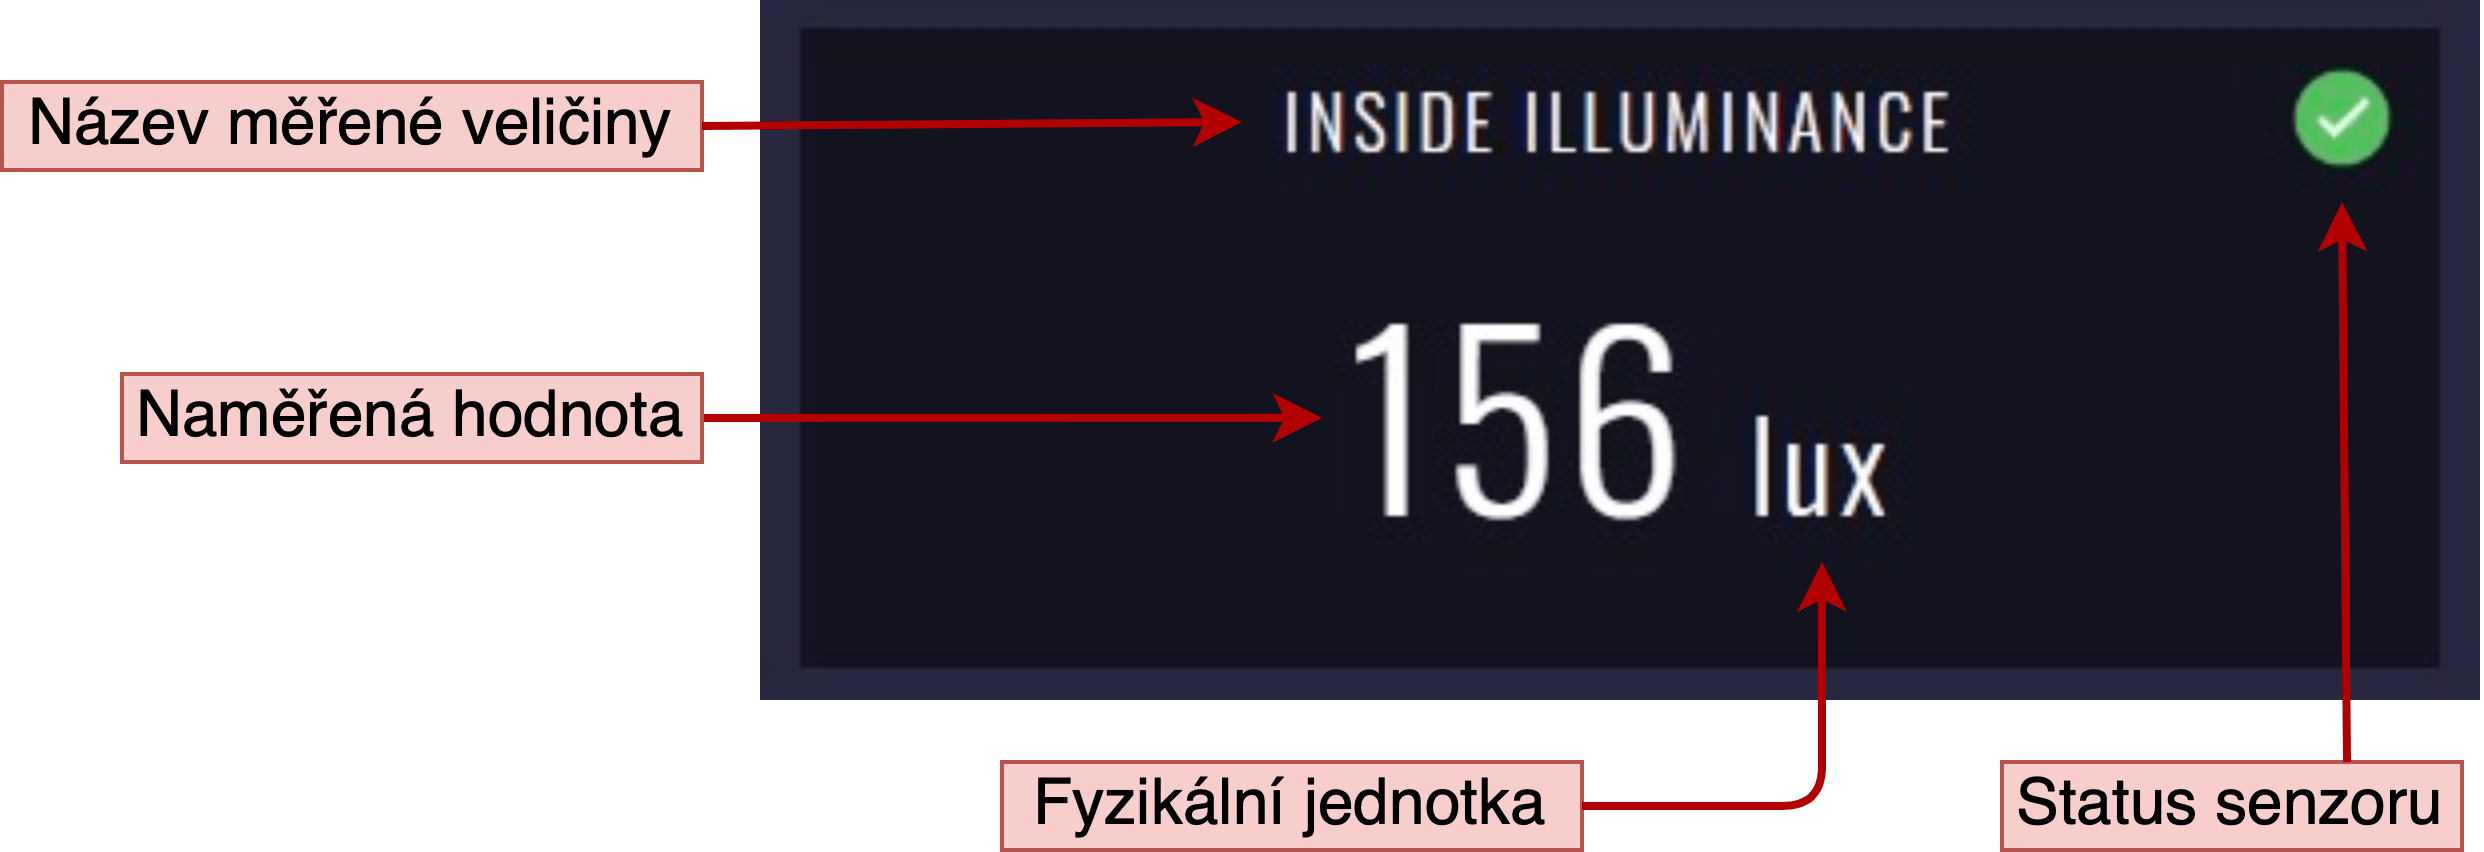
\includegraphics[width=0.7 \textwidth]{web_overview_tile.png}
  \caption{Detail dlaždice na stránce Overview}
  \label{fig:web_overview_tile}
\end{figure}

Ikona v pravém horním rohu dlaždice se mění podle statusu senzoru. Status senzoru může nabývat tří hodnot. Jednotlivé ikony jsou na \cref{fig:web_overview_icons} a význam těchto stavů je popsán v \cref{subsec:diagnostics_output}. 

\begin{figure}[H]
  \centering
  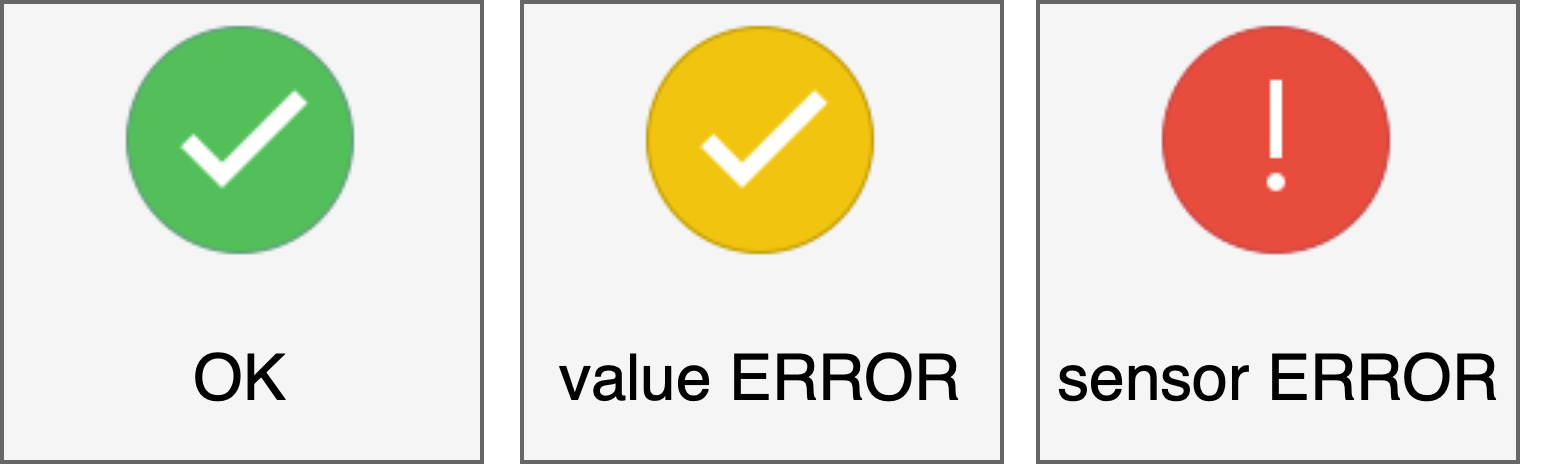
\includegraphics[width=0.45 \textwidth]{web_overview_icons.png}
  \caption{Zobrazení všech ikon popisujících stavy senzoru}
  \label{fig:web_overview_icons}
\end{figure}

Záměrem stránky Overview je neustálý přísun aktuálních dat bez nutnosti jakékoliv obsluhy. Tato stránka může být otevřená nonstop na monitoru a uživatel díky ní má okamžitý přehled o veškerém dění v chytré domácnosti. Na stránku se pomocí protokolu Websocket (více v \cref{sec:websocket}) automaticky propisují nejnovější data bez nutnosti obnovy webu. Účelem je uživatele uceleně informovat o aktuálních hodnotách měřených veličin v chytré domácnosti.

\section{Analytics} \label{sec:analytics}

Stránka Analytics umožňuje výběr konkrétní měřené veličiny a nabízí náhled na grafy očekávaného vývoje, které jsou tvořeny na základě natrénovaného modelu. Prvním krokem po vstupu do sekce Analytics je výběr z předvoleb v horizontálním panelové sekci pod hlavním menu. Po vyplnění všech předvoleb dostane uživatel informace o daném senzoru a zobrazí se graf ilustrující očekávané denní hodnoty dané veličiny na základě klasifikace pomocí natrénovaného modelu (klasifikace je popsána v \cref{sec:classifier})

\begin{figure}[H]
  \centering
  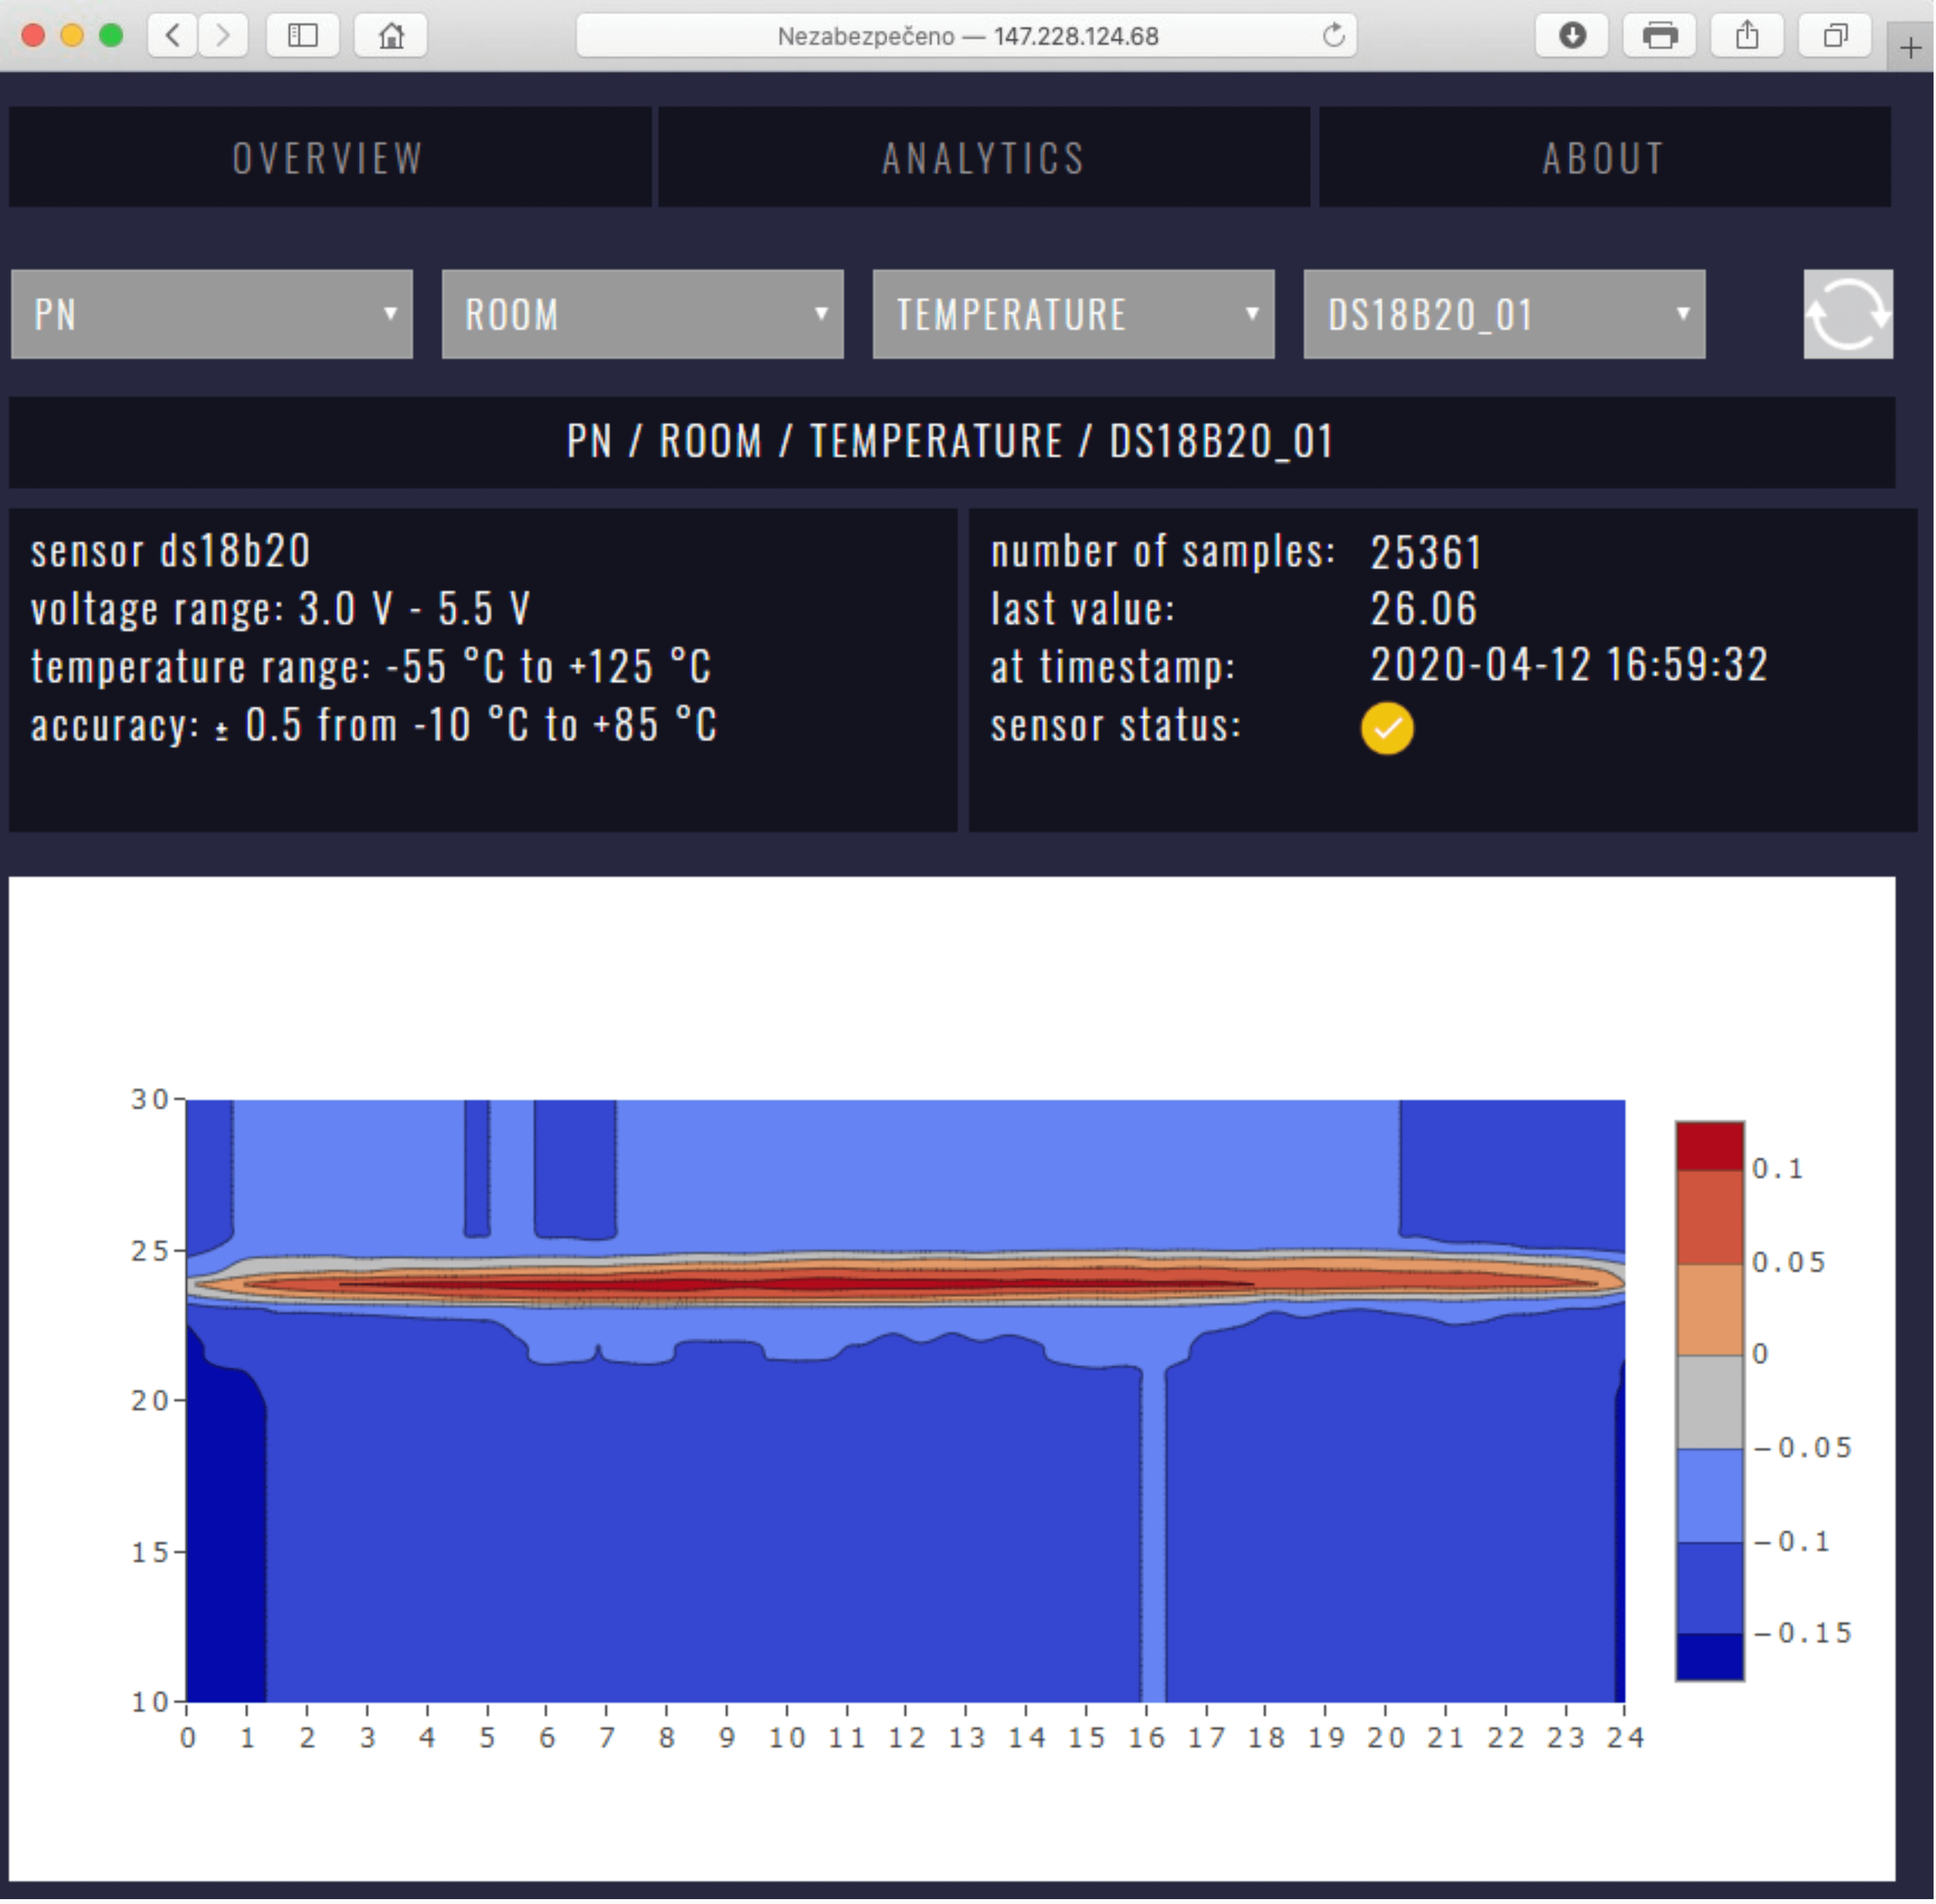
\includegraphics[width=0.9 \textwidth]{web_analytics1.png}
  \caption{Stránka Analytics ve webovém rozhraní}
  \label{fig:web_analytics1}
\end{figure}

Výběr z předvoleb v horizontální sekci probíhá zleva doprava. Uživatel musí nejprve zvolit vlastníka senzoru. Dokud nezvolí vlastníka, nemá možnost kliknout na další políčka. Po volbě vlastníka senzoru zvolí umístění senzoru (opět dokud nezvolí lokaci, nemá možnost kliknout na tlačítko "Quantity"). Po volbě lokace vybere fyzikální veličinu, jejíž data chce zobrazit. Konečně po volbě veličiny vybere konkrétní senzor, který měří zvolenou fyzikální veličinu. Po vyplnění tlačítka ("Sensor ID") se volba odešle na server a pod panelovou sekcí se zobrazí požadovaná data. Poslední tlačítko v panelové sekci vpravo slouží k vyresetování předem zadaných voleb. Po kliknutí na toto tlačítko dostane uživatel možnost vybrat například jinou fyzikální veličinu, která ho zajímá, aniž by musel obnovovat celou stránku. Předvolby, které uživatel volí, se mění v průběhu procesu výběru - například pokud uživatel zvolí jako lokaci "room", v dalším kroku se mu nabídnou pouze fyzikální veličiny, které jsou měřeny v rámci místnosti. Pokud jako lokaci vybere "outside", v dalším kroku se mu zobrazí možnost vybrat pouze fyzikální veličiny ve venkovním prostřední (v tomto případě venkovní teplota). Proces specifikace voleb je znázorněn na \cref{fig:web_analytics_choose}. Stejným způsobem funguje poslední volba na tlačítku "Sensor ID". Množina senzorů, které je možno v tomto tlačítku vybrat je kompletně závislá na všech předešlých volbách - uživatel musí zvolit vlastníka, lokaci a měřenou veličinu, aby bylo možné určit senzory, které splňují tyto podmínky. Na \cref{fig:web_analytics_choose} byl zvolen vlastník \textit{PN}, lokace \textit{ROOM}, veličina \textit{TEMPERATURE} a v poslední volbě "Sensor ID"\ je možné vybrat jen \textit{DS18B20\_01} nebo \textit{BME280\_01}, protože pouze tyto dvě čidla jsou od vlastníka PN a měří teplotu v místnosti.

\begin{figure}[H]
  \centering
  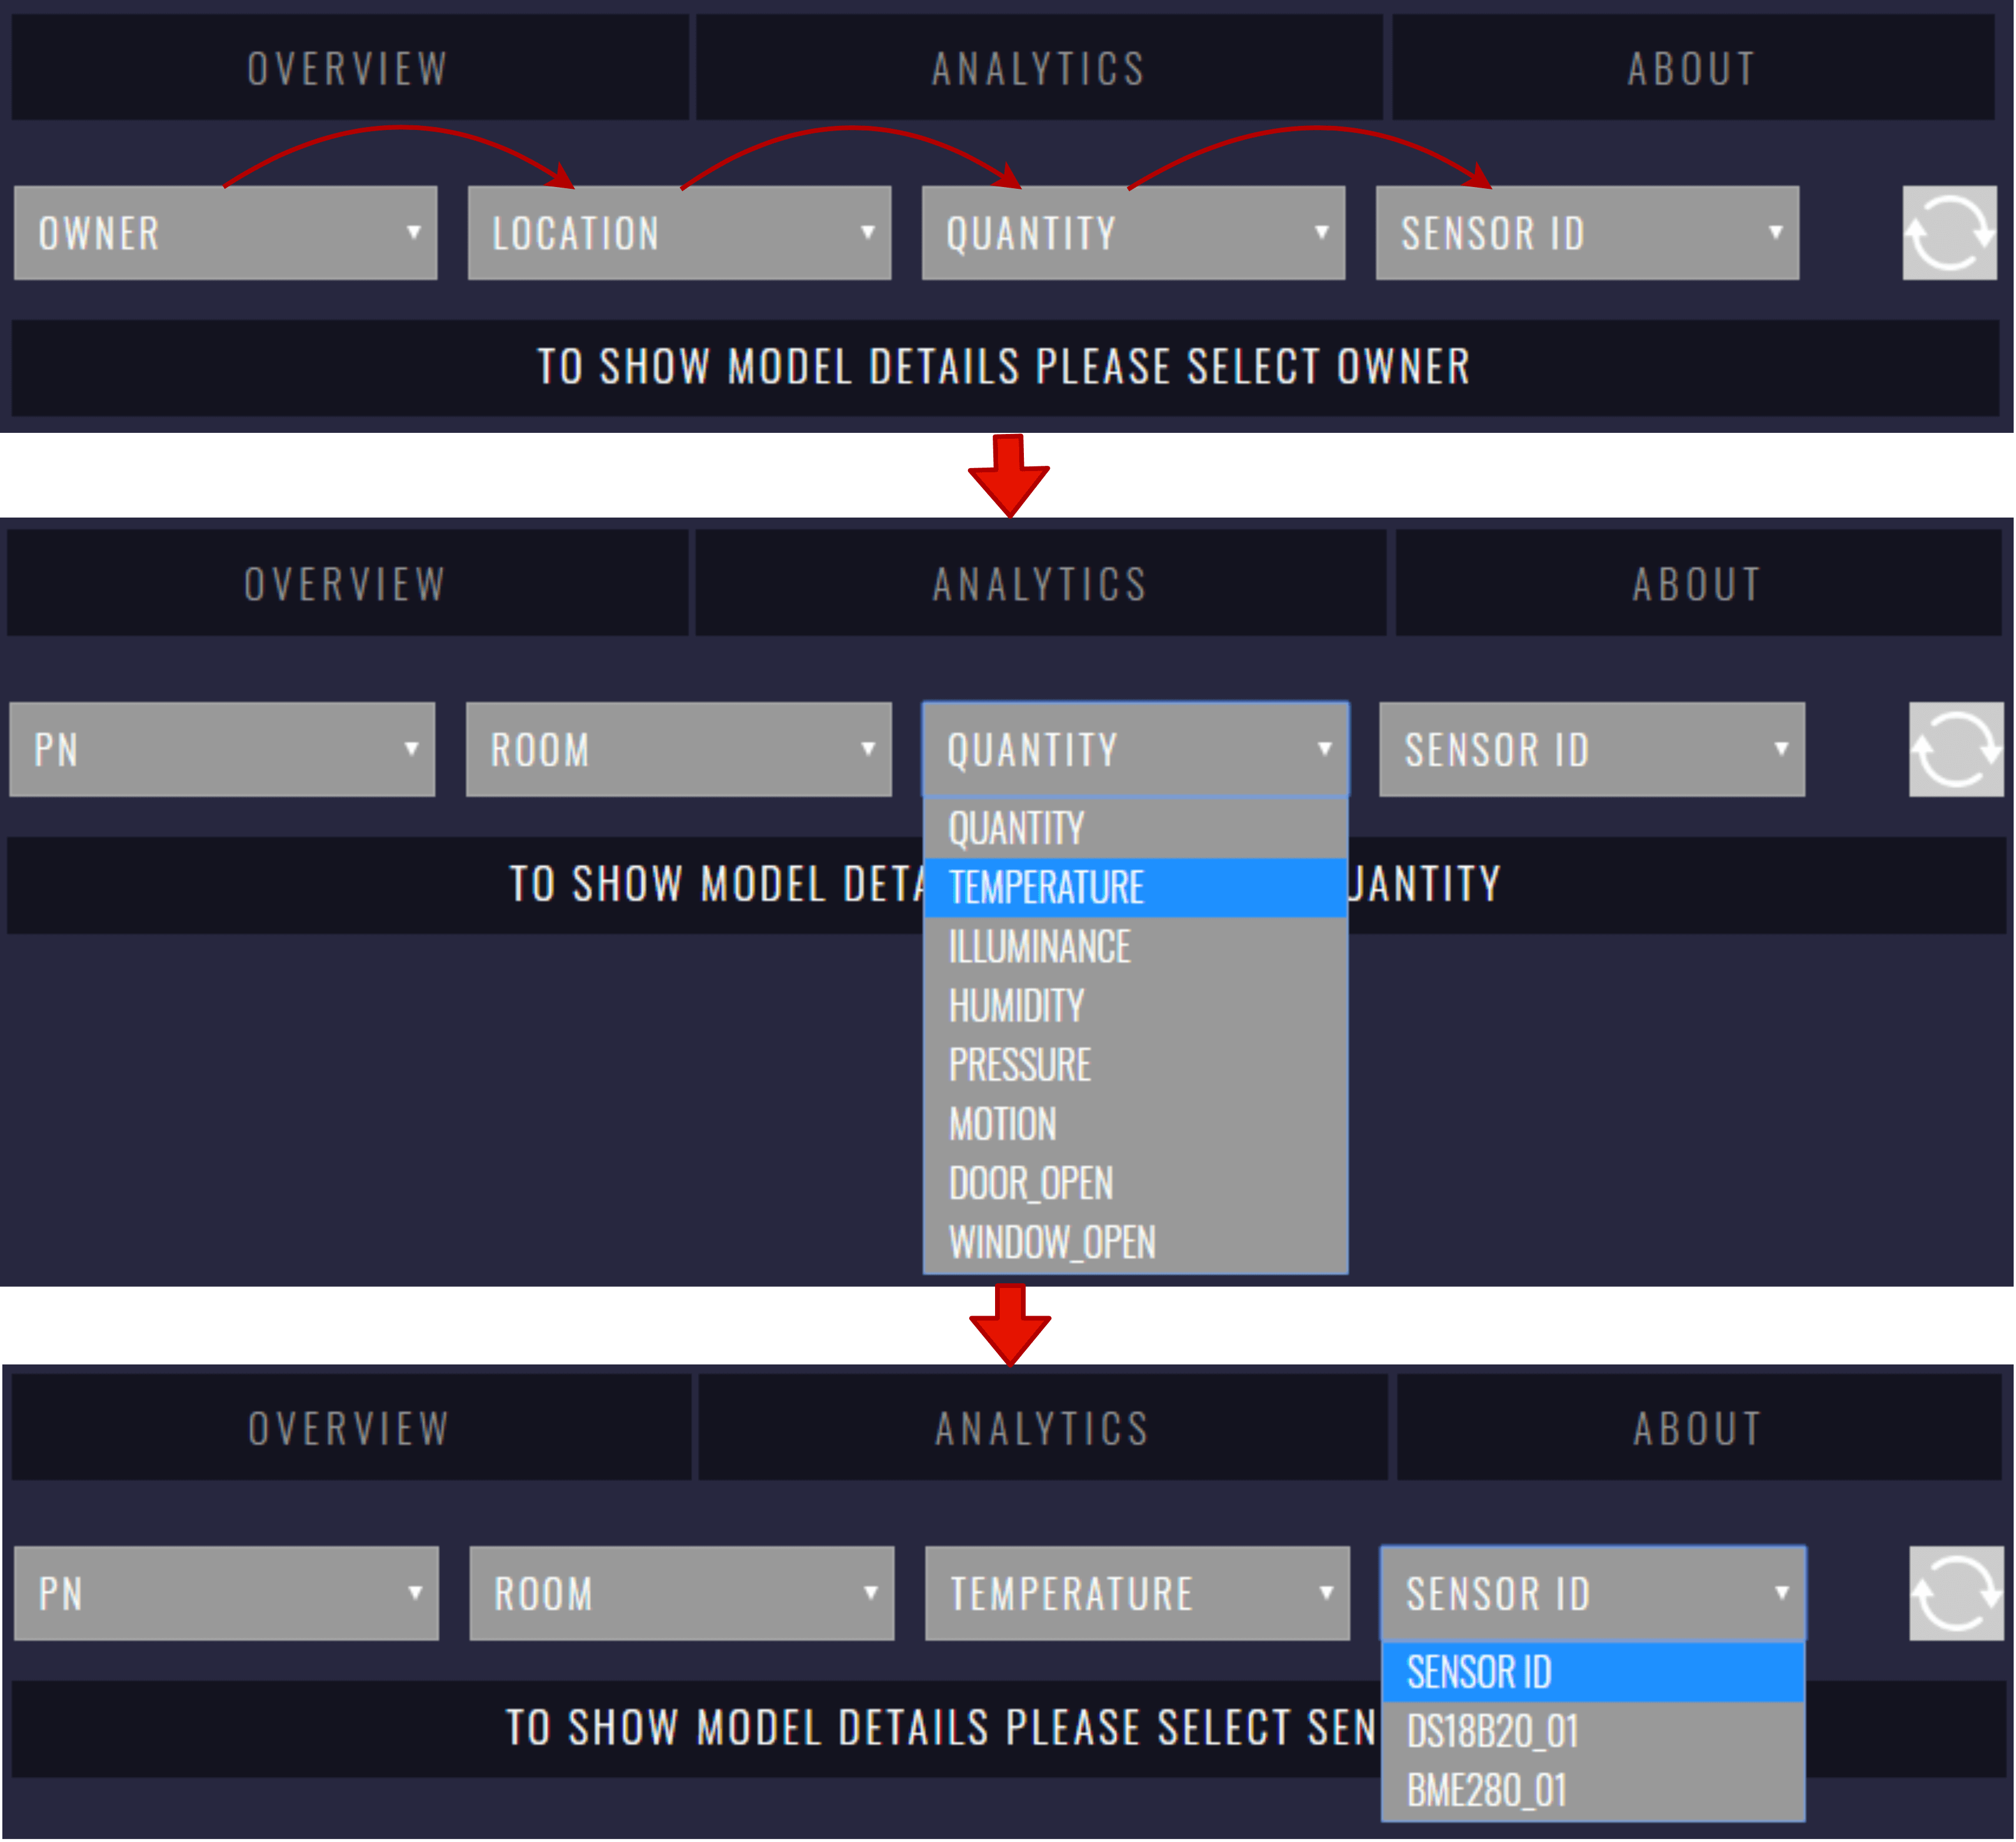
\includegraphics[width=0.9 \textwidth]{web_analytics_choose.png}
  \caption{Proces výběru z předvoleb a specifikace zobrazení dat}
  \label{fig:web_analytics_choose}
\end{figure}

Na \cref{fig:web_analytics_description} jsou popsány jednotlivé dlaždice na stránce Analytics. Po uživatelské volbě všech vstupních parametrů je pod panelovou sekcí zobrazena specifikace zvoleného čidla, v levé dlaždici uprostřed stránky je stručný popis parametrů daného čidla, vedle se nacházejí základní informace o čidlu a ve velké dlaždici jsou zobrazeny očekávané hodnoty na základě statistik natrénovaného modelu pro danou fyzikální veličinu (více v \cref{sec:classifier}). V dlaždici s informacemi o naměřených hodnotách dostane uživatel stručný přehled o datech ze senzoru - kolik vzorků dat se nachází v databázi, jaká byla poslední hodnota, kdy byla tato hodnota naměřena a konečně status senzoru.

\begin{figure}[H]
 \centering
  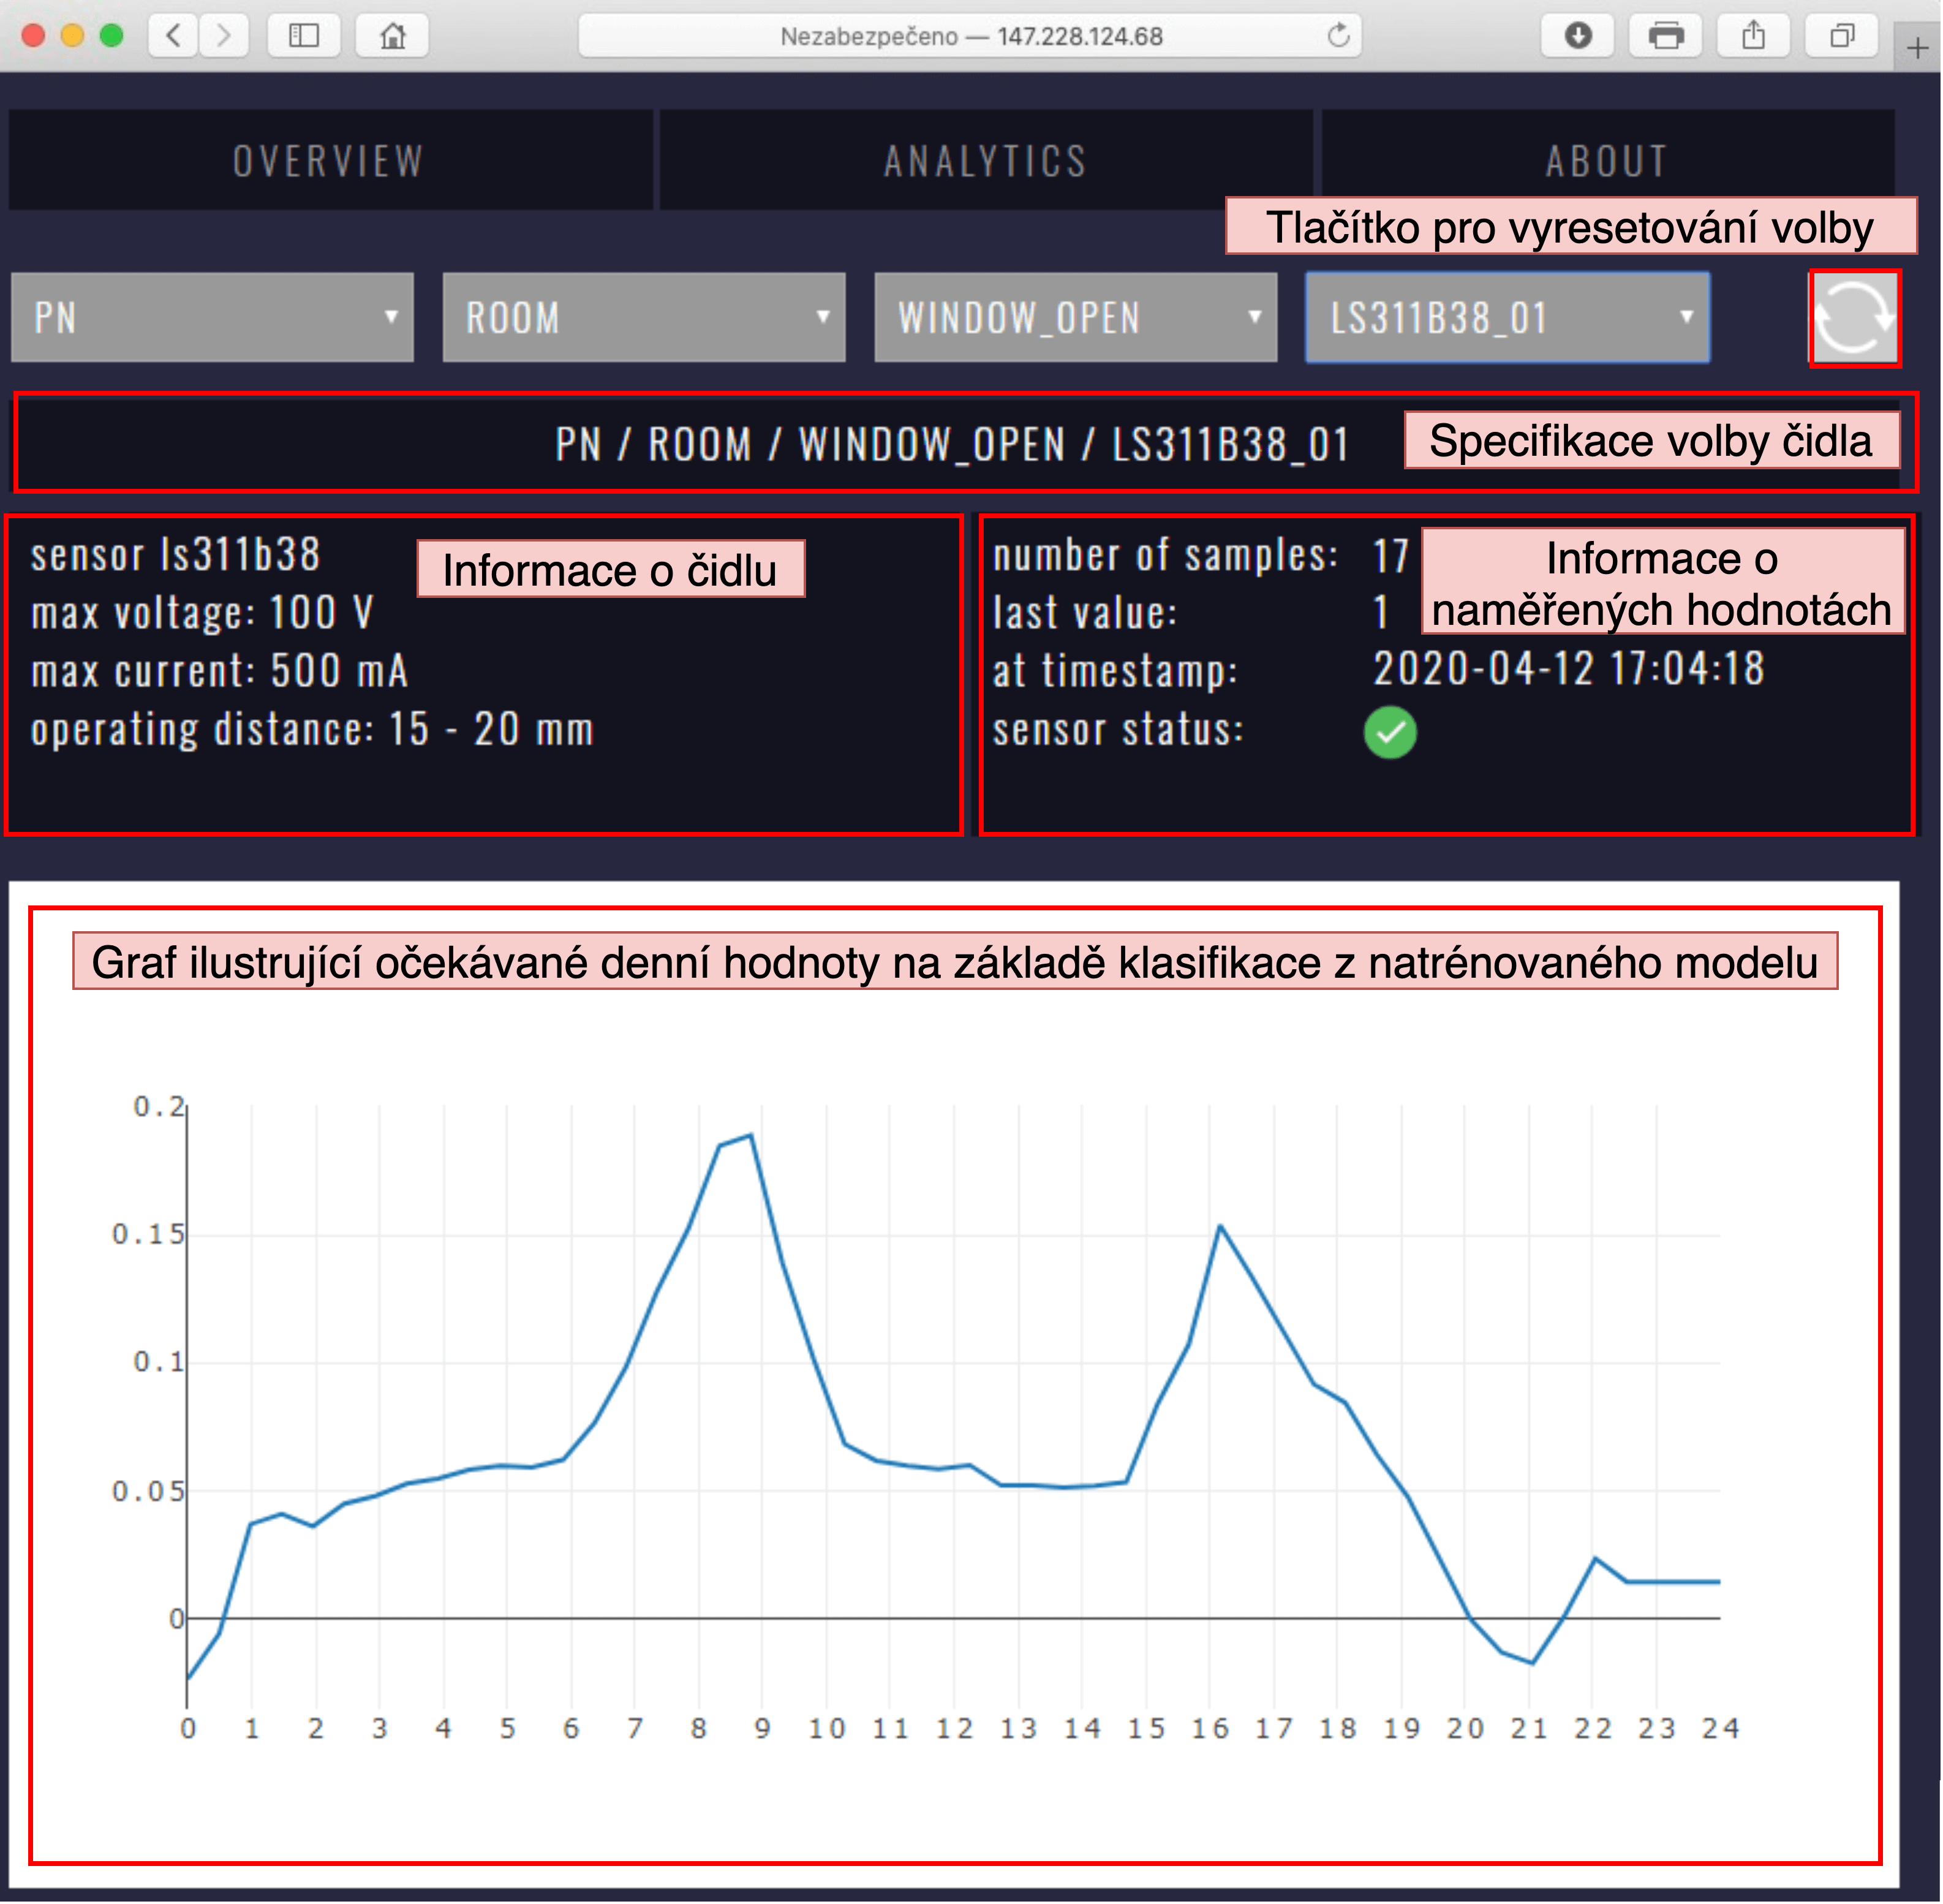
\includegraphics[width=0.9 \textwidth]{web_analytics_description.png}
  \caption{Popis jednotlivých dlaždic na stránce Analytics}
  \label{fig:web_analytics_description}
\end{figure}

\section{About} \label{sec:about}

About je doplňující stránka, která poskytuje stručné informace o projektu a vysvětlivky k používaným ikonám. Na \cref{fig:web_about} je zobrazena kompletní stránka About. 

\begin{figure}[H]
  \centering
  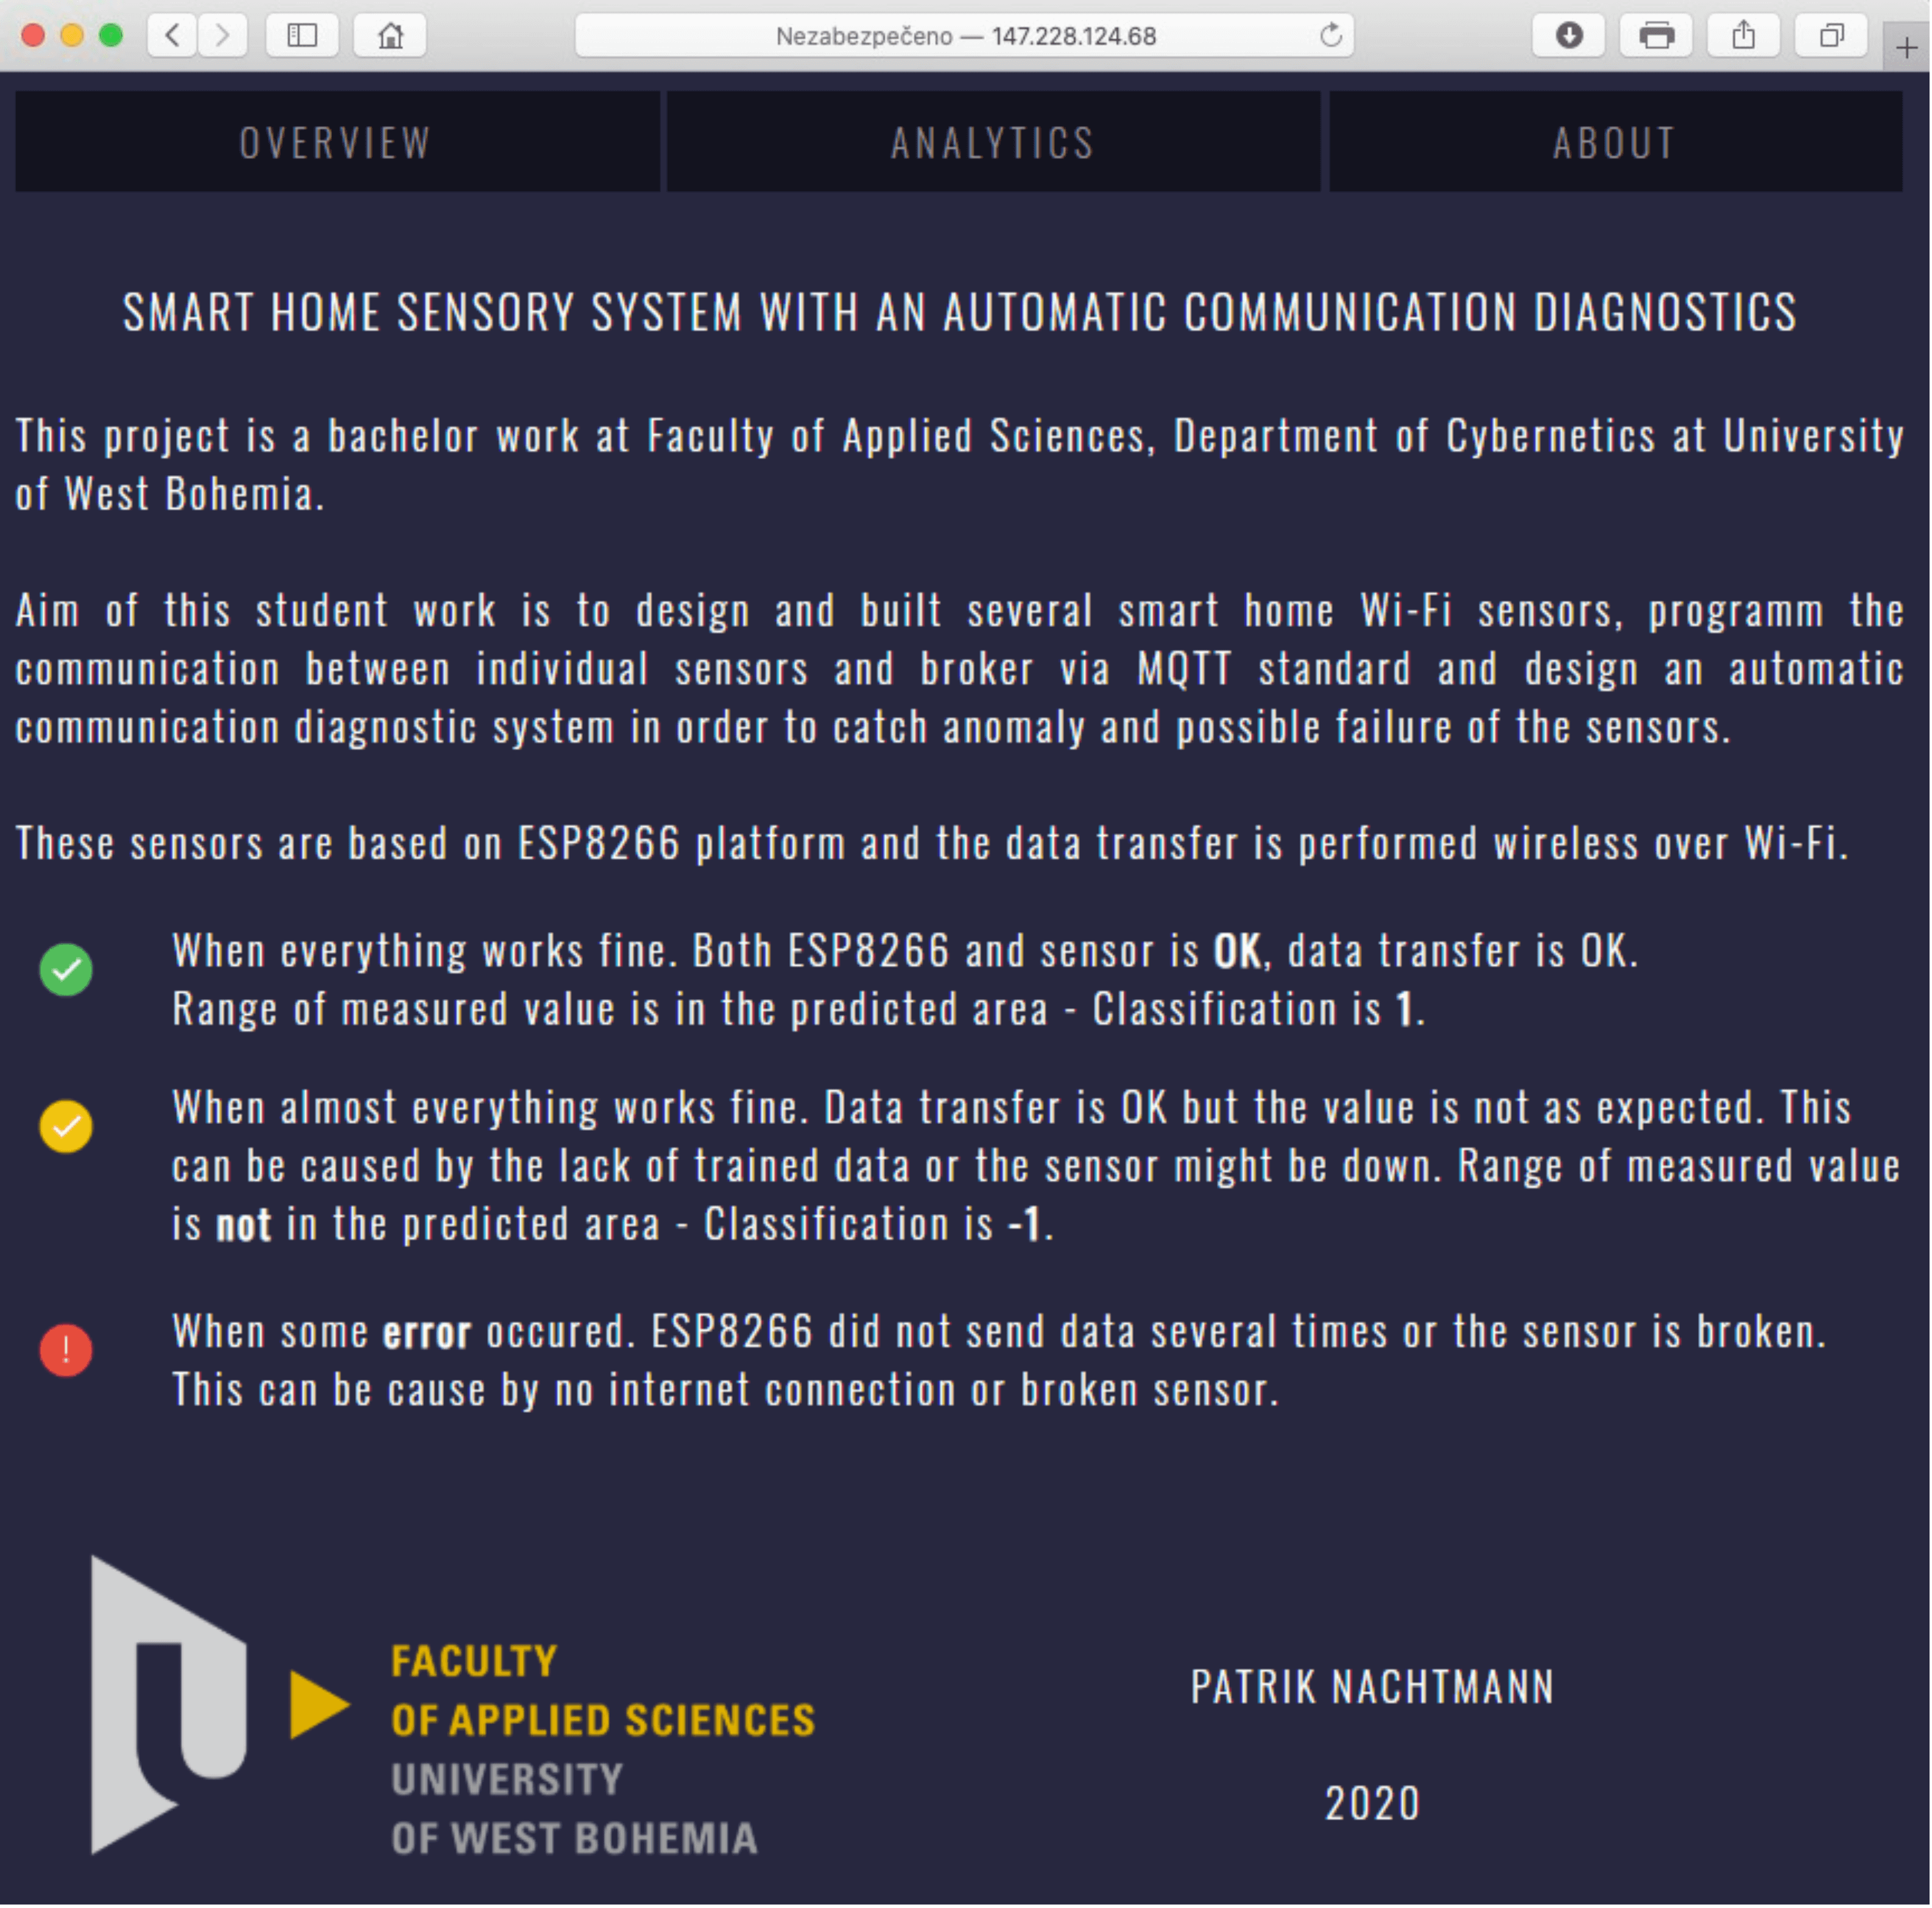
\includegraphics[width=0.9 \textwidth]{web_about.png}
  \caption{Stránka About ve webovém rozhraní}
  \label{fig:web_about}
\end{figure}

Celá webová vizualizace byla navržena tak, aby nabízela jak stručný a výstižný pohled na aktuální dění v chytré domácnosti, tak pokročilý náhled na měřené veličiny s možností vykreslení grafů budoucího vývoje, které slouží primárně pro představu o klasifikaci dalších zpráv, ale i například k vytvoření představy o tom, jak se měřená veličina vyvíjí v čase. 